\documentclass[a4paper]{article}
\usepackage[english]{babel}
\usepackage[utf8x]{inputenc}
\usepackage[T1]{fontenc}
\usepackage{listings}
\usepackage[a4paper,margin=2cm]{geometry}
\usepackage{amsmath}
\usepackage{graphicx}
\usepackage[colorinlistoftodos]{todonotes}
\usepackage[colorlinks=true, allcolors=blue]{hyperref}
\usepackage{wasysym} % smileys
\usepackage{fancyhdr}
\usepackage{tikz}
\usetikzlibrary{arrows}
\setlength\parindent{0pt} % indent


% my commands:
\newcommand{\n}{\newline}
\newcommand{\tab}{\hspace{1cm}}

\begin{document}

\renewcommand{\headrulewidth}{0pt} % removes horizontal bars from headers and footers
\thispagestyle{fancy} % beware the difference between \thispagestyle and \pagestyle
\lhead{9.1}
\rhead{Vilém Zouhar}

\section*{NORkování}
Již víme, že libovolnou hradlovou síť umíme popsat pomocí operátorů NEG, OR, AND. Bude tedy stačit, pokud pomocí NOR popíšeme tyto operátory.

\subsection*{NEG}
Jednoduše zapojíme vstup do NOR.

\begin{center}
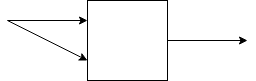
\includegraphics[width=4cm]{neg}
\end{center}

\section*{OR}
X, Y zapojíme do NOR a výstup znegujeme.

\begin{center}
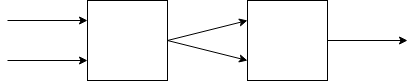
\includegraphics[width=6cm]{or}
\end{center}


\section*{AND}
X, Y znegujeme a výstupy zapojíme do NOR. Toto (a OR) je nejhlubší realizace, tudíž je to horní odhad na zvětšení jakékoliv booleovské hradlové sítě (hloubka ze zvětší dvakrát).
\begin{center}
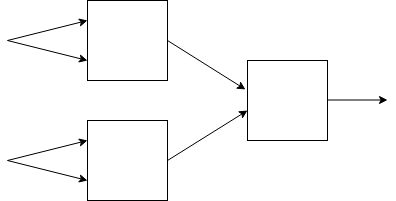
\includegraphics[width=7.5cm]{and}
\end{center}


\subsection*{NORkování z NANDávání}
Předchozí část problém již řeší, nicméně pokud přijmeme fakt, že NAND je s konstantami univerzální, pak nám stačí, pokud NOR převedeme na NAND. Přikládám to, neboť je to opravdu zadarmo z předchozího AND:


\begin{center}
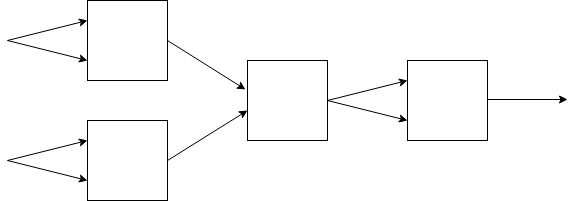
\includegraphics[width=9cm]{nand}
\end{center}



\end{document}